\scanpage{16}
\figure{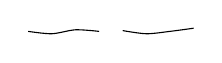
\begin{tikzpicture}\draw plot[smooth] coordinates {(0,0) (.3,-.03) (.6,.02) (.9,0)};\draw plot[smooth] coordinates {(1.2,.01) (1.5,-.03) (1.8,0) (2.1,.04)};\end{tikzpicture}}
Frobénius itéré : notation $p_S^\nu(X)$, $\operatorname{Frob}_S^\nu(X)$.
Les développements précédents sont valables, en \unsure{changeant} les
puissances \unsure{$p$ième} par les puissances $p^\nu$-ièmes.
\figure{\begin{tikzpicture}\draw plot[smooth] coordinates {(0,0) (.3,.07) (.6,-.01) (.9,0)};\draw (1.2,.02) .. controls (1.4,-.03) .. (1.7,0);\draw (1.9,.03)--(2,.0);\draw (2.3,.02)--(2.4,0);\end{tikzpicture}}

Cas d'un préschéma de \uline{base parfait}.
On dira que $S$ est \uline{parfait} si \deleted{\unsure{son}}
$\mathcal O_S\mathbin{\overset{\operatorname{Frob}(S)^*}{\text{---}}}\mathcal O_S$
est un \uline{isomorphisme}.
Le cas le plus important est celui où $S$ est le spectre d'un corps, où
la terminologie coïncide avec celle usuelle.

\uline{Dans ce cas}, \uline{le préschéma} $p_S^\nu(X)$ est
\uline{isom au préschéma} $X$ \uline{par} $\mathrm{pr}_1$, \uline{mais}
\uline{on se rappellera que ce n'est pas un} $S$-\uline{isom}.
\uline{En général}, $p_S^\nu(X)$ \uline{n'est pas}
$S$-\uline{isom à} $X$.
\figure{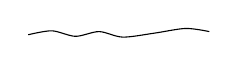
\begin{tikzpicture}\draw plot[smooth] coordinates {(0,0) (.3,.05) (.6,-.02) (.9,.04) (1.2,-.03) (1.6,.02) (2,.08) (2.3,.04)};\end{tikzpicture}}

Cas d'un corps de base fini, à $q=p^{\unsure{h|\nu}}$ éléments.
\inserted{$[\deleted{\unsure{\nu=h\nu}}\unsure{\nu\mapsto h\nu}]$}
Alors $\operatorname{Frob}_{\unsure{S}}^{h\nu}(S):S\longrightarrow S$
est l'identité. Donc \uline{pour de tels} $\nu$,
\deleted{\unsure{le} \illegible{2}}\inserted{le morphisme can}
$p_S^\nu(\unsure{X})\mathbin{\text{---}}X$ \uline{est un} $S$-\uline{isom}.
Donc on peut considérer $\operatorname{Frob}_S^{h\nu}(X)$ comme un
\mspage{15}
